%!TEX program = xelatex
\documentclass[11pt,a4paper,UTF8,fontset=fandol]{ctexart}

\usepackage[a4paper,margin=2.0cm]{geometry}
\usepackage{amsmath,amssymb}
\usepackage{booktabs}
\usepackage{graphicx}
\usepackage{xcolor}
\usepackage{hyperref}
\usepackage{microtype}
\usepackage{tikz}
\usepackage{pgfplots}
\usepgfplotslibrary{groupplots}
\usetikzlibrary{arrows.meta,calc,positioning}
\pgfplotsset{compat=1.18}

\definecolor{sourceblue}{HTML}{1F4E79}
\definecolor{derivegreen}{HTML}{276221}
\definecolor{warnred}{HTML}{9C0006}
\definecolor{boxgray}{HTML}{F3F5F7}
\definecolor{qmcblue}{HTML}{0072B2}
\definecolor{tanorange}{HTML}{D55E00}
\definecolor{mutedgray}{HTML}{5B6570}

\hypersetup{
  colorlinks=true,
  linkcolor=sourceblue,
  citecolor=derivegreen,
  urlcolor=sourceblue,
  pdftitle={TFIM SSE-QMC 方法与基准说明},
  pdfauthor={HarnessingQuantum-2026}
}

\setlength{\parindent}{2em}
\setlength{\parskip}{0.35em}
\setlength{\emergencystretch}{3em}

\pgfplotstableread[col sep=comma]
  {data/tfim-l2-validation-note-data.csv}\LTwoData
\pgfplotstableread[col sep=comma]
  {data/tfim-l4-validation-note-data.csv}\LFourData

\pgfplotsset{
  benchmark axis/.style={
    width=0.93\textwidth,
    height=5.7cm,
    axis line style={line width=0.9pt},
    tick style={line width=0.8pt},
    tick label style={font=\small},
    label style={font=\large},
    title style={font=\large\bfseries},
    grid=major,
    grid style={draw=gray!22,line width=0.5pt},
    legend style={
      draw=none,
      fill=none,
      font=\small,
      cells={anchor=west},
      at={(0.02,0.04)},
      anchor=south west
    }
  }
}

\title{\textbf{TFIM 的 SSE-QMC：方法、学习过程与基准}}
\author{HarnessingQuantum-2026}
\date{2026-07-30}

\begin{document}
\maketitle

\section{两句话说明方法与代码来源}

本项目采用 fixed-length stochastic series expansion（SSE）：在
\(\sigma^z\) 基底中直接抽样 \(\exp(-\beta H)\) 的 Taylor 算符串，
diagonal update 改变展开阶数，TFIM 专用 quantum-cluster update 联合改变传播
自旋和 \(D_i\leftrightarrow F_i\)，因此没有离散虚时间带来的 Trotter 误差
\cite{Sandvik2003,Sandvik2019}。

当前 Julia SSE 代码主要由 AI 完成；我通过持续追问、核对公式和阅读代码，初步学习了
operator string、细致平衡、linked vertices、cluster update 与能量估计量的想法，
但不把这等同于已经独立从零重写算法。代码的可信度来自下面的 deterministic tests、
精确小系统检查和跨方法 benchmark，而不是来自“AI 生成”或“程序能够运行”本身。

\paragraph{采样和能量。}
每个 \(\beta\) 使用多个独立随机种子；先丢弃 warmup，再把测量 sweeps 分箱，
由独立 bins/replicas 给出均值和 Monte Carlo standard error（MCSE）。若
\(n\) 是非单位算符数，\(n_0\) 是可解析的 \(hI\) 算符数，代码使用
\[
m=n-n_0,\qquad
\frac{E}{N}=\frac{J N_b-\langle m\rangle/\beta}{N}.
\]
它与标准式
\((J N_b+hN-\langle n\rangle/\beta)/N\) 完全等价，只是去掉了已知的独立
Poisson 噪声，不引入近似。

\section{经典 quantum-cluster 更新图}

图~\ref{fig:cluster-update} 直接采用 Sandvik 讲义的 Fig.~3(b)：左半是翻转前，
右半是翻转后。绿色线不是临时挑选的若干轨迹，而是由全部 vertices 和虚时间
links 确定的一个完整 cluster。

\begin{figure}[htbp]
\centering
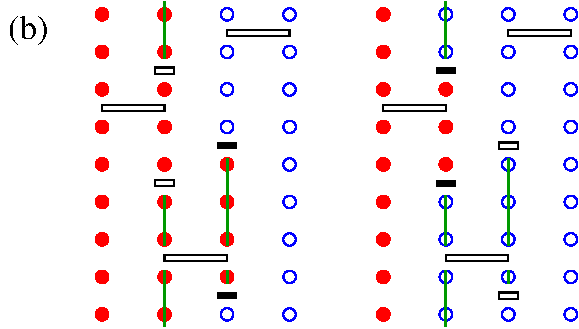
\includegraphics[width=0.96\textwidth]{sandvik-2019-fig3b.pdf}
\caption{Sandvik 讲义 Fig.~3(b) 的原始图像裁剪，未重画。绿色 cluster 被整体翻转；
相应自旋腿改变，并使部分 site vertices 在 diagonal 与 off-diagonal 类型之间转换。
来源：Sandvik, \emph{Stochastic Series Expansion Methods},
Fig.~3(b)\cite{Sandvik2019}。}
\label{fig:cluster-update}
\end{figure}

\clearpage
\section{\texorpdfstring{\(2\times2\)}{2x2}：ED、SSE 与 tanTRG}

\begin{figure}[htbp]
\centering
\begin{tikzpicture}
\begin{groupplot}[
  group style={group size=1 by 2,vertical sep=1.35cm},
  benchmark axis,
  xmin=1,xmax=10
]
\nextgroupplot[
  ylabel={$E/N$},
  xticklabels=\empty,
  title={$2\times2$ OBC TFIM,\quad $J=1,\ h=0.5$}
]
\addplot[black,line width=1.5pt]
  table[x=beta,y=ed_energy] {\LTwoData};
\addlegendentry{ED}
\addplot[
  qmcblue,only marks,mark=diamond*,mark size=2.7pt,
  error bars/.cd,y dir=both,y explicit
] table[x=beta,y=qmc_energy,y error=qmc_mcse] {\LTwoData};
\addlegendentry{SSE-QMC $\pm1$ MCSE}
\addplot[
  tanorange,line width=1.3pt,mark=o,mark size=2.6pt,
  mark options={fill=white,line width=1.0pt}
] table[x=beta,y=tantrg_energy] {\LTwoData};
\addlegendentry{tanTRG}

\nextgroupplot[
  xlabel={$\beta J$},
  ylabel={$\lvert\Delta E\rvert/\lvert E_{\rm ED}\rvert$},
  ymode=log,
  ymin=1e-14,ymax=1e-3,
  log basis y=10
]
\addplot[qmcblue,only marks,mark=diamond*,mark size=2.7pt]
  table[x=beta,y=qmc_relative] {\LTwoData};
\addlegendentry{SSE deviation}
\addplot[qmcblue,dashed,line width=1.3pt]
  table[x=beta,y=qmc_mcse_relative] {\LTwoData};
\addlegendentry{SSE 1-MCSE}
\addplot[
  tanorange,line width=1.3pt,mark=o,mark size=2.5pt,
  mark options={fill=white,line width=1.0pt}
] table[x=beta,y=tantrg_relative] {\LTwoData};
\addlegendentry{tanTRG deviation}
\end{groupplot}
\end{tikzpicture}
\caption{\(2\times2\) 精确小系统基准。每个温度使用 20 个独立 replicas；
\(\beta=1,2\) 每个 replica 使用 \(2^{21}\) measurement sweeps，其余温度使用
\(2^{18}\)。所有 SSE 点均在 ED 的 \(3\) MCSE 内，最大
\(\lvert z\rvert=1.98\)；tanTRG 与 ED 的最大相对差约为
\(4\times10^{-14}\)。}
\label{fig:l2-validation}
\end{figure}

\clearpage
\section{\texorpdfstring{\(4\times4\)}{4x4}：SSE 与 tanTRG}

\begin{figure}[htbp]
\centering
\begin{tikzpicture}
\begin{groupplot}[
  group style={group size=1 by 2,vertical sep=1.35cm},
  benchmark axis,
  xmode=log,
  xmin=0.015,xmax=10
]
\nextgroupplot[
  ylabel={$E/N$},
  xticklabels=\empty,
  title={$4\times4$ OBC TFIM,\quad $J=1,\ h=0.5$}
]
\addplot[
  tanorange,line width=1.3pt,mark=o,mark size=2.5pt,
  mark options={fill=white,line width=1.0pt}
] table[x=beta,y=tantrg_energy] {\LFourData};
\addlegendentry{tanTRG}
\addplot[
  qmcblue,only marks,mark=diamond*,mark size=2.7pt,
  error bars/.cd,y dir=both,y explicit
] table[x=beta,y=qmc_energy,y error=qmc_mcse] {\LFourData};
\addlegendentry{SSE-QMC $\pm1$ MCSE}

\nextgroupplot[
  xlabel={$\beta J$},
  ylabel={$\lvert\Delta E\rvert/\lvert E_{\rm SSE}\rvert$},
  ymode=log,
  ymin=1e-6,ymax=1e-1,
  log basis y=10
]
\addplot[
  tanorange,line width=1.3pt,mark=o,mark size=2.5pt,
  mark options={fill=white,line width=1.0pt}
] table[x=beta,y=tantrg_relative] {\LFourData};
\addlegendentry{tanTRG deviation}
\addplot[qmcblue,dashed,line width=1.3pt]
  table[x=beta,y=qmc_mcse_relative] {\LFourData};
\addlegendentry{SSE 1-MCSE}
\end{groupplot}
\end{tikzpicture}
\caption{\(4\times4\) 的 25 个共同 \(\beta\) 点，未做插值。SSE 主网格每个温度
使用 20 replicas、每个 replica \(2^{18}\) measurement sweeps；高温扩展使用
\(2^{22}\)。tanTRG--SSE 的最大标准化偏差为
\(\lvert z\rvert=2.04\)，未出现超过 \(3\) MCSE 的点。高温处能量接近零，
因此相对偏差会放大，应同时参考 MCSE。}
\label{fig:l4-validation}
\end{figure}

\section{结论与团队分工}

图~\ref{fig:l2-validation} 对照 ED 检查小系统的绝对正确性，
图~\ref{fig:l4-validation} 检查尺寸增大后 SSE 与独立 tanTRG 的一致性。
它们支持“当前实现通过了已测试模型和参数范围内的 benchmark”，但不等价于对任意
Hamiltonian、尺寸和参数都无错误的数学证明。

这部分 SSE baseline 的代码与学习过程主要由本人和 AI 协作完成；后续更强的测试与
独立交叉检查由\textbf{高建鑫}和\textbf{许传书}完成。提交材料中应保留这一分工，
同时把 QMC 统计误差与 tensor-network 截断误差分开报告。

\begin{thebibliography}{9}

\bibitem{Sandvik2003}
A.~W. Sandvik,
\newblock Stochastic series expansion method for quantum Ising models with
arbitrary interactions,
\newblock \emph{Physical Review E} \textbf{68}, 056701 (2003).

\bibitem{Sandvik2019}
A.~W. Sandvik,
\newblock Stochastic Series Expansion Methods,
\newblock arXiv:1909.10591 (2019).

\end{thebibliography}

\end{document}
